% Chapter 4

\chapter{Prototypation} % Main chapter title

\label{Chapter4} % For referencing the chapter elsewhere, use \ref{Chapter4} 

%----------------------------------------------------------------------------------------

\section{Early version}

This version is very simple and it contains only the basic functionalities. 
The goal of this version are: understand if this kind of system can be useful for the users, and experiment some technical solutions to create the features needed to achieve the goals. At this stage the application is evidently incomplete, there are numerous deficiencies and inconsistencies and the goals of the Human Machine Interaction are ignored. All this point are corrected in the second version, and this first version is used to show a "before-after comparison".
GAn Web is a web application (as the name suggests) so the interface is created using HTML and CSS. This languages are very advanced and allows the programmer to create and modify an interface very easily. The framework Bootstrap, used in this project, even improve the performances of these languages. So all the prototypes are directly created by code, without paper-based mock ups.

Following are visible some part of the early prototype, with very simple features.

\begin{enumerate}
\item The homepage:

\begin{figure}[H]
\centering
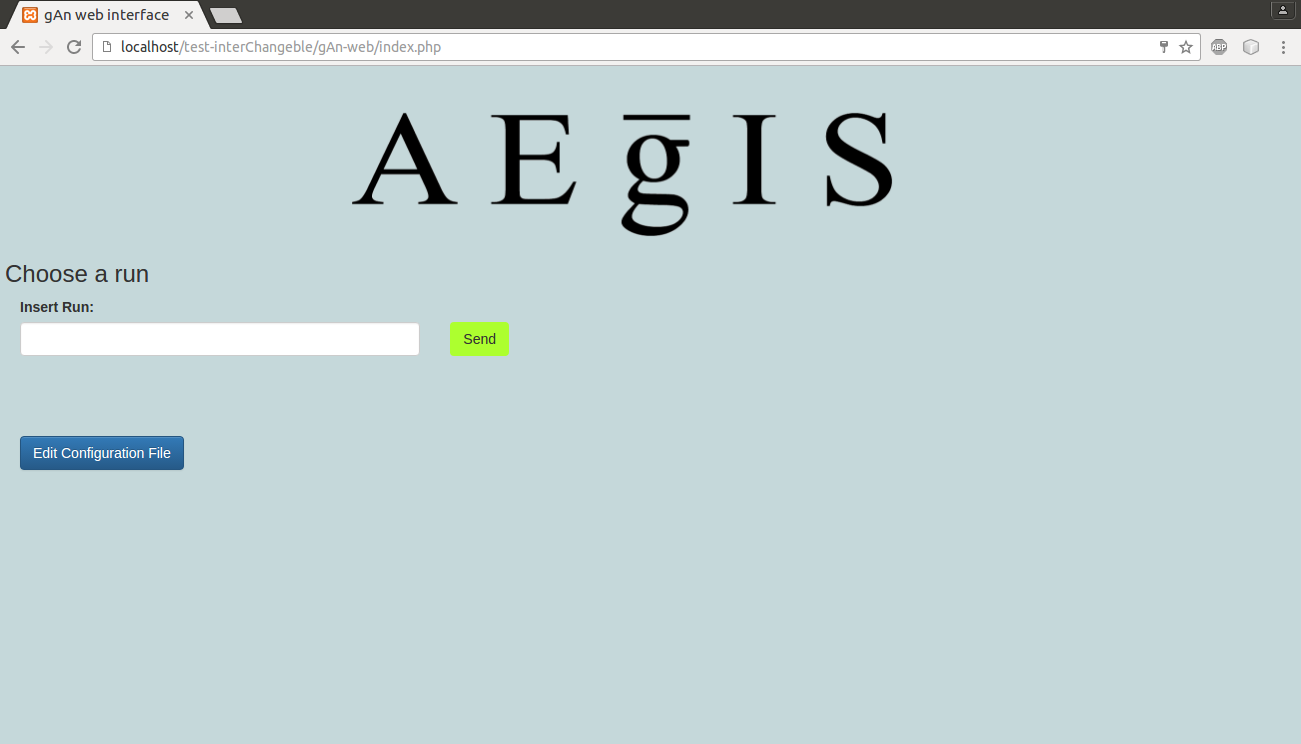
\includegraphics[scale=0.5]{HomePageOLD.png} 
\caption{The early homepage of gAn Web}
\end{figure}

It is quite clear: There is the AEgIS Logo, an input field where the user can insert a run number (only one in this version) and a "Send" button to start the analysis (using gAn). A button "Edit Configuration File" allows the user to  enter in the page dedicated to the configuration of the program.

\item The text output page:

\begin{figure}[H]
\centering
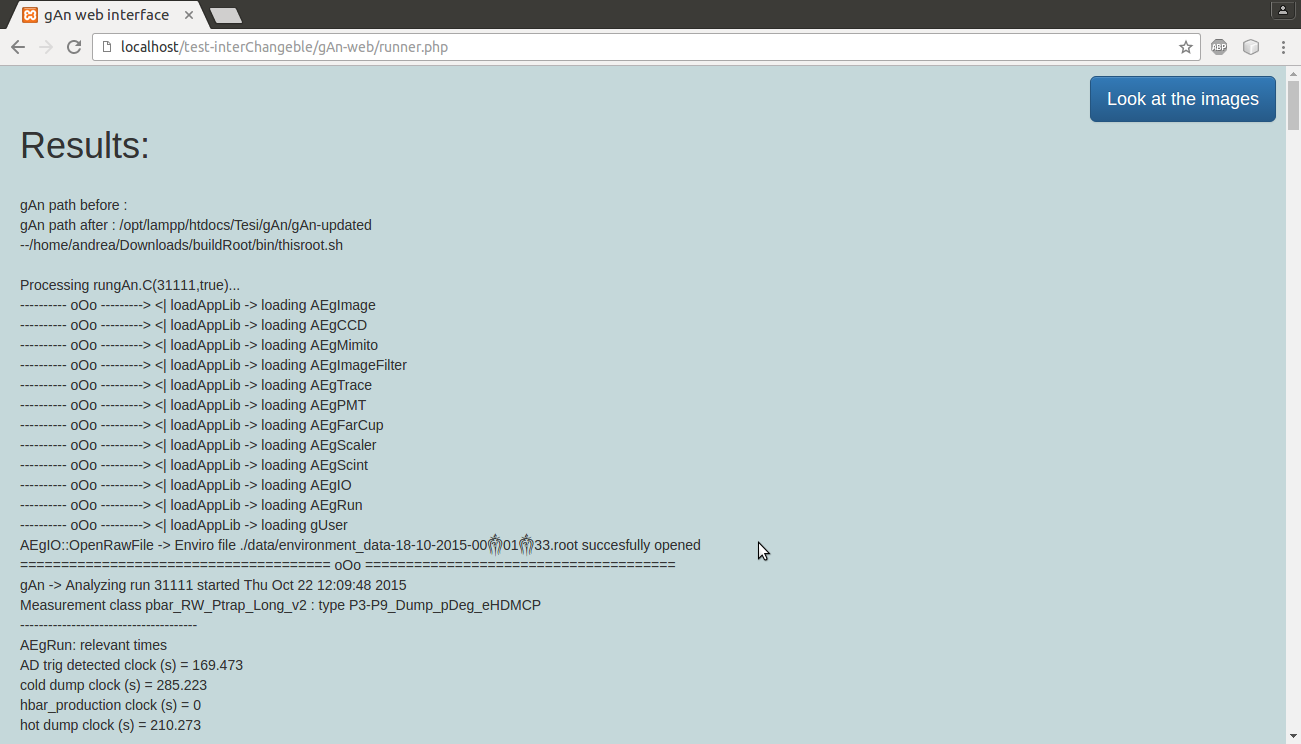
\includegraphics[scale=0.5]{TextOutputOLD.png} 
\caption{The early page related to the textual output of gAn Web}
\end{figure}
  
The textual result of the computation is visible: it seems to be too long and incomprehensible, but for physicists it is quite clear. The graphics is very minimalist, there is only one button: "Look at the images", that sends the user to the page related to the images. 



\item The page related to the images:

\begin{figure}[H]
\centering
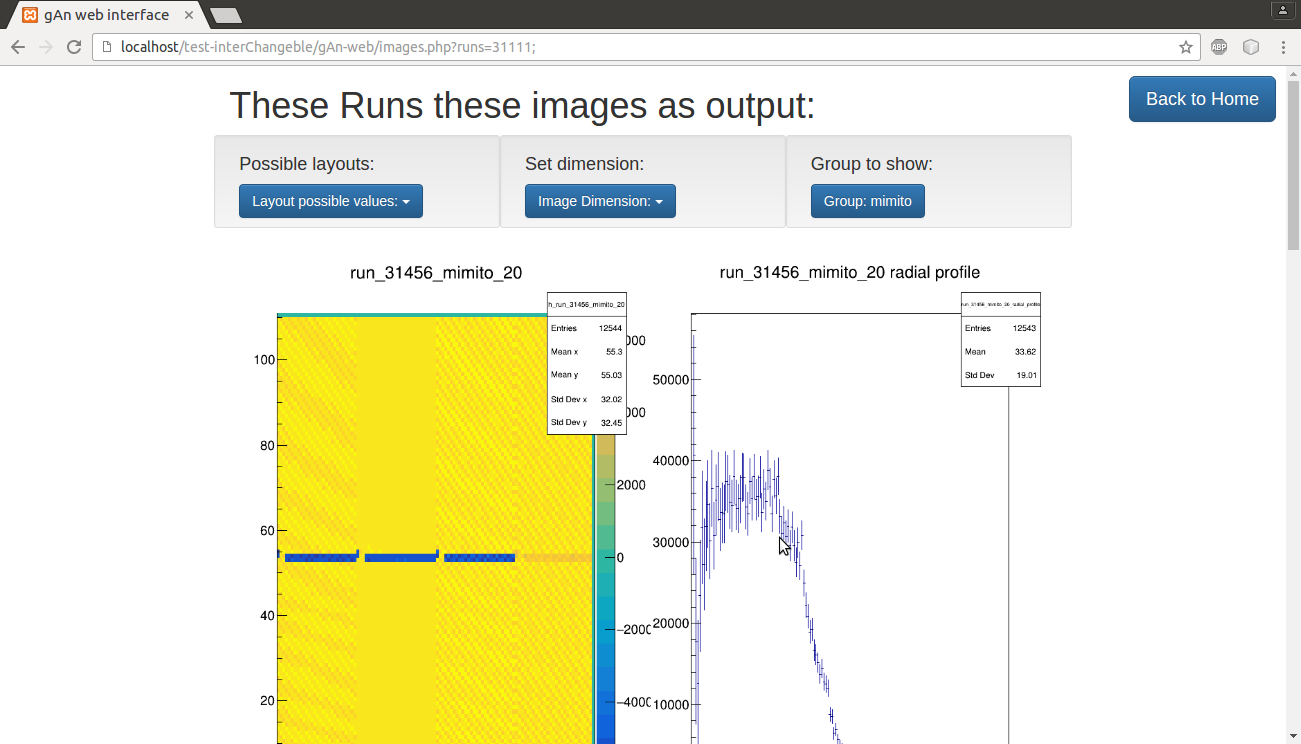
\includegraphics[scale=0.5]{AllImagesOLD.png} %TODO %TODO %TODO %TODO %TODO %TODO %TODO %TODO %TODO %TODO %TODO %TODO %TODO %TODO %TODO %TODO %TODO %TODO %TODO %TODO %TODO %TODO %TODO %TODO %TODO %TODO %TODO %TODO %TODO %TODO %TODO %TODO %TODO %TODO %TODO %TODO %TODO %TODO %TODO %TODO %TODO %TODO %TODO %TODO %TODO %TODO %TODO %TODO %TODO %TODO %TODO %TODO %TODO %TODO SISTEMA STOCAZZO DI IMMAGINE
\caption{The page able to show the output images in the early prototype}
\end{figure}   

This page shows the images in a dynamic framework, that the user can edit.
The user the chose by dropdown menus the dimension, the layout ("vertical", if he prefers the images disposed vertically one above the other, "carousel" if he prefers the images organized horizontally, navigable by a "next" button and a "previous" button), the group to show (each image belongs to a group, each group usually is composed by 2-3 images). Clicking on a image the user can open it in a full page version (but it is still a static image, a png).



\item The page that aims to edit the configuration file:

\begin{figure}[H]
\centering
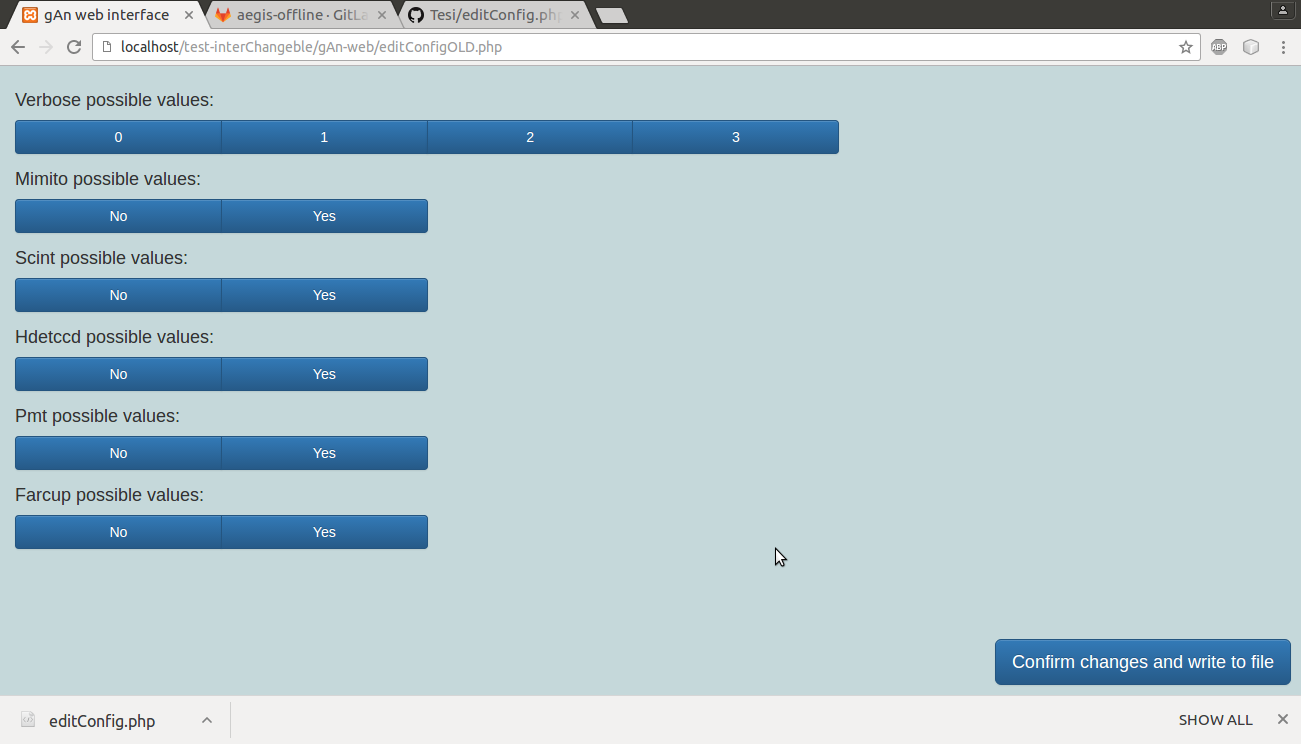
\includegraphics[scale=0.5]{EditConfigOLD.png} %TODO %TODO %TODO %TODO %TODO %TODO %TODO %TODO %TODO %TODO %TODO %TODO %TODO %TODO %TODO %TODO %TODO %TODO %TODO %TODO %TODO %TODO %TODO %TODO %TODO %TODO %TODO %TODO %TODO %TODO %TODO %TODO %TODO %TODO %TODO %TODO %TODO %TODO %TODO %TODO %TODO %TODO %TODO %TODO %TODO %TODO %TODO %TODO %TODO %TODO %TODO %TODO %TODO %TODO PROCURA LA CAZZO DI IMMAGINE CON I RADIOBUTTONS 
\caption{The configuration page}
\end{figure}   

This page allows the user to chose by radio buttons (modified using Bootstrap graphic) the value to insert in the configuration file of gAn. Radio buttons force users to insert correct values.    

\end{enumerate}

\section{How the early version can be improved}
The early version's goal is just to be a demo. In particular, it is based on the assumption that the user knows in every moment all about gAn (how does it works,  what is the meaning of each field of the configuration file, etcetera). It can be improve literally in every point, according with the principles of the Human Machine Interaction.

\subsection{Modified pages}

\subsection{Added pages}

\section{Late version}
